\documentclass{article}
\usepackage{graphicx}
\usepackage[french]{babel}
\usepackage{multicol}
\usepackage{geometry}
\usepackage{titling}
\usepackage[utf8]{inputenc}
\usepackage{natbib}
\usepackage[style=authoryear,backend=biber]{biblatex}
\usepackage[colorlinks=true,linkcolor=blue,citecolor=green,urlcolor=red]{hyperref}

\usepackage{float}
\usepackage{fancyhdr}

\addbibresource{name.bib}

\geometry{
    a4paper,
    total={170mm,257mm},
    left=20mm,
    top=30mm,
}

% Set up the fancy header and footer
\pagestyle{fancy}
\fancyhf{}
\fancyfoot[C]{Page \thepage}

\title{
    
\includegraphics[width=1\textwidth]{photo/UCLouvain_Charleroi.png} \\
    \vspace{1.5cm}
    {\Huge \textbf{Rapport Personnel \\ Projet Bite2Meet}} \\
    \vspace{1.5cm}
}

\author{
    \textbf{Moussaoui Noah} \\
    Université catholique de Louvain-la-Neuve \\
    Campus de Charleroi, EPL en SINC \\
    Délégué et ambassadeur \\
    \texttt{Noah.moussaoui@student.uclouvain.be}
}

\date{
    \vspace{1.5cm}
    Durée de recherche : Septembre - Novembre \\
    \vspace{1.5cm}
    
\includegraphics[width=0.5\textwidth]{photo/EPL.png}
}

\begin{document}

\maketitle
\newpage

\section{Introduction}
Dans le cadre de ce projet, nous avons développé une application mobile innovante destinée aux requins souhaitant interagir avec d'autres requins dans un cadre social et compagine pour la chasse . 
Contrairement aux applications traditionnelles de rencontres, notre solution se positionne comme un réseau social. 
Elle permet aux utilisateurs de se connecter pour organiser des chasses humaines, consulter des publications, participer à des événements, et visionner des stories. 

Nous nous sommes basés sur les données d' un fichier CSV contenant des informations détaillées 
sur diverses attaques de requins dans le monde. 
Ces données alimentent notre application et permettent de proposer une expérience utilisateur
pertinente et immersive. Nous allons les étudiers plus précisement dans la suite de ce rapport 
dans la partie \hyperref[sec:data]{"Data asbstraction"}

\section{Personas}
Voici les différents personas représentant des profils typiques de clients potentiels de notre 
application. 

\subsection*{Perona : Acheteur}
\subsubsection{Bob Fisher (Persona de Nizar)}
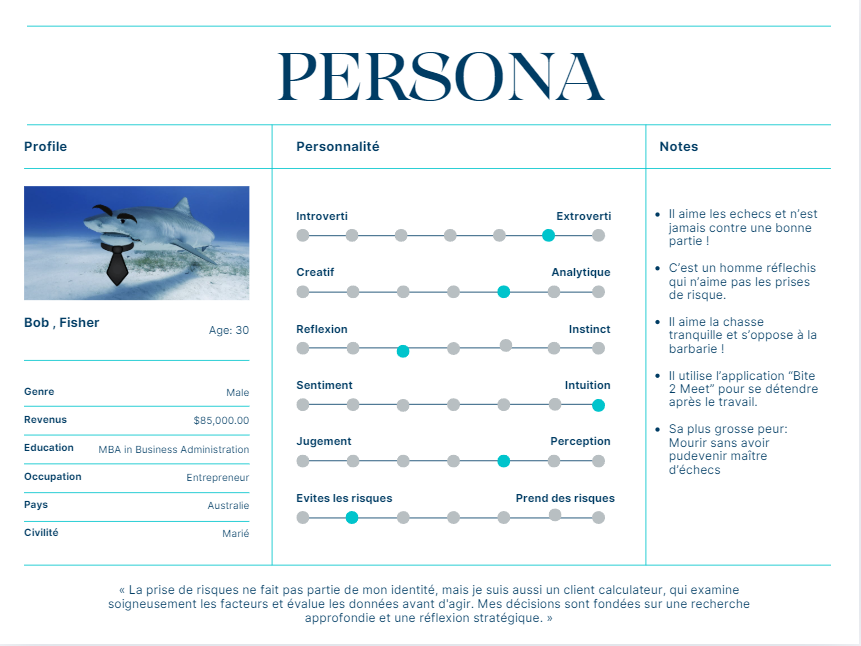
\includegraphics[width=1\textwidth]{photo/Persona_Nizar.png}\\

Bob Fisher, entrepreneur australien visionnaire, a identifié une opportunité unique sur le marché 
des réseaux sociaux et des applications mobiles. Passionné par la chasse entre amis et les classements 
des meilleurs chasseurs, il a imaginé une plateforme innovante où les requins pourraient se connecter
pour organiser des chasses humaines près de chez eux, avec d’autres passionnés partageant les mêmes 
intérêts, et ce, à travers le monde entier.\\

En tant qu’homme très fortuné, Bob souhaite également intégrer une section premium à l’application, 
destinée aux utilisateurs les plus aisés. Cette fonctionnalité exclusive offrirait des options
avancées, telles que la possibilité de naviguer anonymement sur le site et de participer à 
des activités privées, tout en garantissant un haut niveau de confidentialité et d’exclusivité.

\subsection{Personas: Client}
\subsubsection*{Sharko Zie (Mon Persona)}
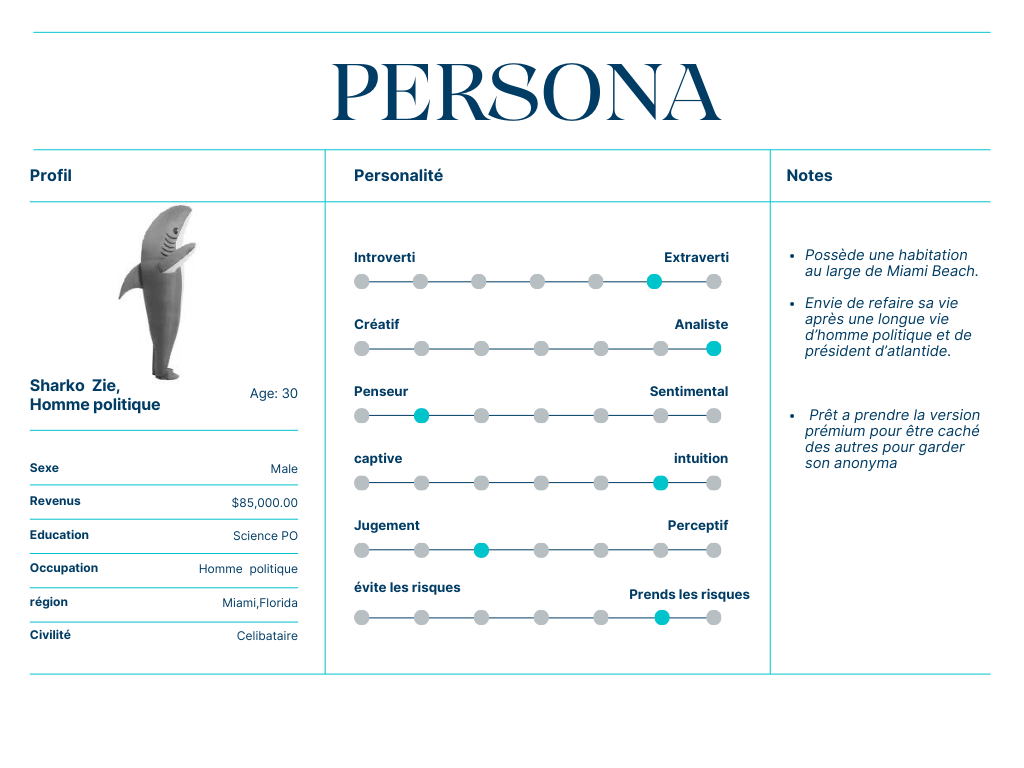
\includegraphics[width=1\textwidth]{photo/Personna_Sharkozie.png}\\

Sharko Zie est un ancien président cherchant à préserver son anonymat tout en explorant de nouvelles 
opportunités sociales. 
Le mode premium de l'application, qui permet de masquer son identité et de modifier sa localisation,
 est une fonctionnalité clé pour lui. 
Lors de ses voyages, Sharko peut ainsi se connecter avec d'autres utilisateurs tout en protégeant
 sa vie privée. 

\subsubsection*{Eric l’Athlète (Persona de Kaan)}
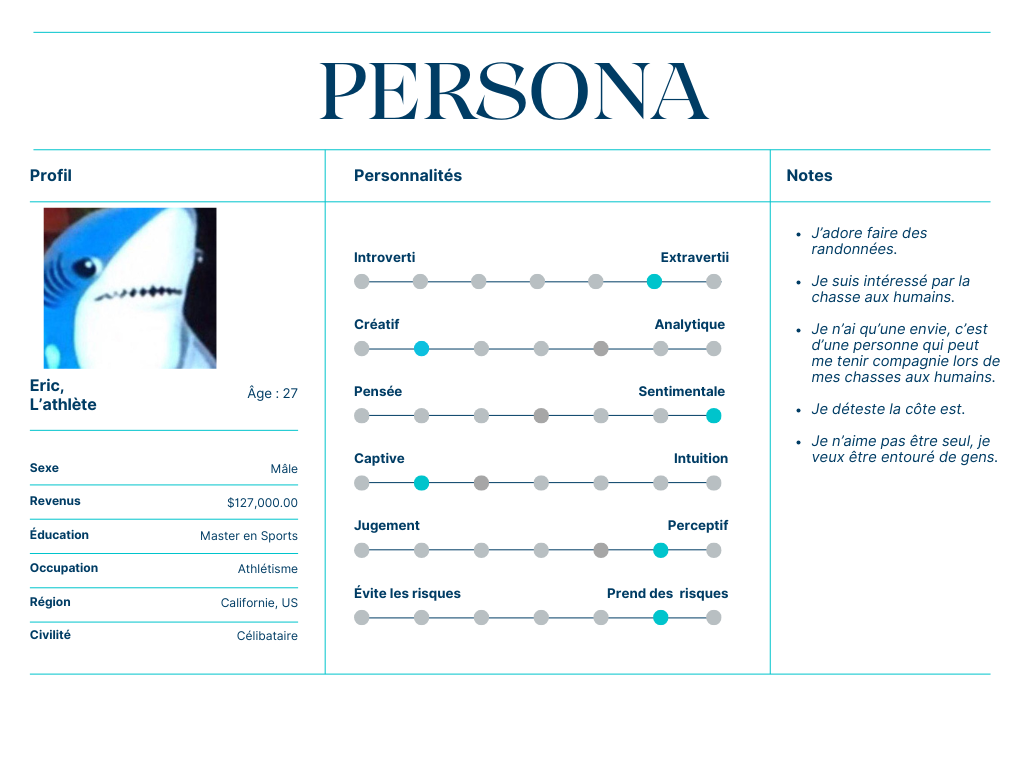
\includegraphics[width=1\textwidth]{photo/Personna_Kaan.png}\\

Eric est un individu très sociable qui aime se connecter avec un grand nombre d’amis et partager 
sa vie à travers des stories et des publications. 
Cependant, il trouve la limite quotidienne d’ajouts d’amis dans la version gratuite contraignante. 
Le mode premium, avec ajout d’amis illimité, répond parfaitement à ses attentes. 
De plus, Eric peut bloquer les utilisateurs d’une région qu’il n’apprécie pas (comme la côte Est) 
pour rendre son expérience plus agréable.



\section{Basse-Fidélité}
Nous avons exploré différentes idées pour les versions basse-fidélité, illustrées par 
les propositions suivantes : 

\includegraphics[width=0.5\textwidth]{photo/tableau.png}

\subsection{Propositions d’idées}
\begin{figure}[H]
    \centering
    \begin{minipage}{0.4\textwidth}
        \centering
        \includegraphics[width=\linewidth]{photo/Alex_basse_fidelité.jpg}
        \caption{Idées d'Alex}
        \label{fig:Alex}
    \end{minipage}
    \hfill
    \begin{minipage}{0.4\textwidth}
        \centering
        \includegraphics[width=\linewidth]{photo/Nizar_basse_fidelité.jpg}
        \caption{Idées de Nizar}
        \label{fig:Nizar}
    \end{minipage}
    \begin{minipage}{0.4\textwidth}
        \centering
        \includegraphics[width=\linewidth]{photo/Kaan_basse_fidelité.jpg}
        \caption{Idées de Kaan (1/2)}
    \end{minipage}
    \hfill
    \begin{minipage}{0.4\textwidth}
        \centering
        \includegraphics[width=\linewidth]{photo/Kaan_basse_fidelité2.jpg}
        \caption{Idées de Kaan (2/2)}
        \label{fig:Kaan}
    \end{minipage}
\end{figure}

Ces idées, discutées lors de nos réunions, ont permis de retenir des éléments essentiels 
et d’identifier des améliorations potentielles. 

\newpage
\subsection{Idées d'Alex}
Dans \hyperref[fig:Alex]{l'idées d'Alex} il propose  de faire une messagerie pour garder
 un contact avec ses amis et les nouvelles rencontres .

\subsection{Idées de Nizar}
Dans \hyperref[fig:Nizar]{l'idées de Nizar} lui a propose une page de réglages permettant de 
modfier le profil, photos mais surtout
d'acceder au prémium et de voir les fonctionnalités possible à réaliser dans l'applis.

\subsection{Idées de Kaan}
Dans \hyperref[fig:Kaan]{l'idées de Kaan} il propose de faire une carte des follewers qui nous suivent et ceux qu'on suit aussi  sur l'appplis ainsi qu'un
réseau qui montre les connexions entre nos amis et les amis de nos amis . Il propose aussi un page de profil où on y trouve 
les infos sur la personne les interets le pourcentage de compatibilité  le classement général de chasse . 



\subsection{Idée générale}
\includegraphics[width=0.5\textwidth]{photo/Visu_basse_fidelité.jpg}\caption{Idée générale}
\label{fig:général}
\vspace{1cm}\\
À la suite des discussions, nous avons abouti à une \hyperref[fig:général]{idée globale}. 
Cette version inclut des fonctionnalités supplémentaires comme :
\begin{enumerate}
    \item Une page de préférences permettant de collecter des informations sur l’utilisateur et de calculer la compatibilité avec d’autres membres.

    \item Une interface de connexion plus intuitive et complète.

    \item Un bouton centralisé de navigation ("hub bouton") offrant un accès rapide aux principales 
    pages de l’application.
\end{enumerate}
Apart ça nous avons amélioré ou gardé les idées de tous le monde . 

\newpage
\section{Data Abstraction}
\label{sec:data}
Nous allons étudier les datas disponibles dans le fichier csv "sharks.csv" le fichier se présente comme ceux ci :



(Détails sur l'abstraction des données à venir…)

\section{Task Abstraction}
(Détails sur l'abstraction des tâches à venir…)

\section{Conclusion}
Ce rapport met en lumière le travail effectué sur le projet, incluant la définition des personas, 
les premières versions basse-fidélité, et une vision globale des fonctionnalités. 
Les prochaines étapes consisteront à affiner les prototypes, intégrer les données, et tester 
les fonctionnalités avec des utilisateurs réels. 

\end{document}
